
\section{Population genetics}

\begin{frame}
        \frametitle{TensorFlow}

        \begin{figure}
        	
\includegraphics[width=0.5\textwidth]{Pics/tensorflow.png}
        \end{figure}

	easy and intuitive way to do ML

\end{frame}

\begin{frame}
        \frametitle{TensorFlow}

        \begin{figure}
                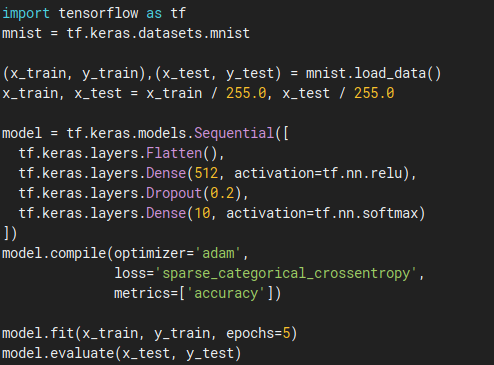
\includegraphics[width=0.5\textwidth]{Pics/tf_code.png}
        \end{figure}

	concept-heavy but code-light

	many parameters, but only few are important to adjust

\end{frame}

\begin{frame}
        \frametitle{TensorFlow}

        \begin{figure}
                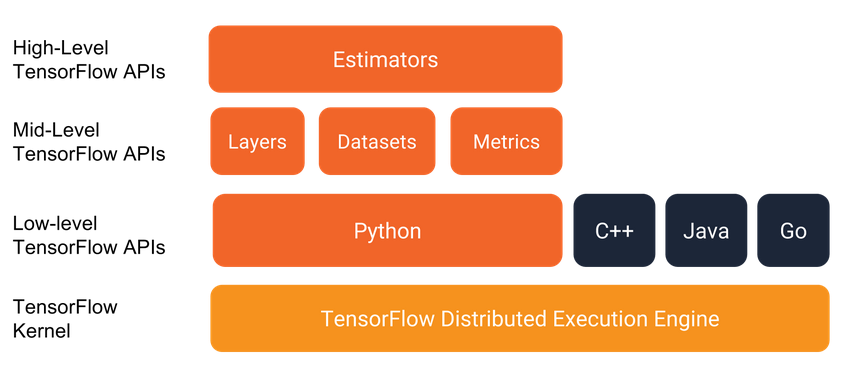
\includegraphics[width=0.9\textwidth]{Pics/tf_api.png}
        \end{figure}

\end{frame}

\begin{frame}
        \frametitle{Low-level APIs}

	What is a tensor?

        \begin{figure}
                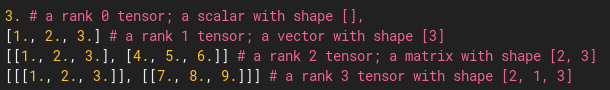
\includegraphics[width=0.7\textwidth]{Pics/tensor.png}
        \end{figure}

	\begin{figure}
                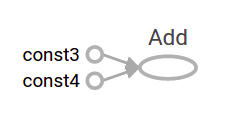
\includegraphics[width=0.4\textwidth]{Pics/graph.png}
        \end{figure}

\end{frame}

\begin{frame}
	\frametitle{Examples of data tensors}

	\begin{itemize}
		\item vector data: 2D tensors of shape \texttt{(samples, features)}
		\item timeseries or sequence data: 3D tensors of shape \texttt{(samples, timesteps, features)}
		\item images: 4D tensors of shape \texttt{(samples, height, width, channels)}
		\item video: 5D tensors of shape \texttt{(samples, frames, height, width, channels)}
	\end{itemize}

	\small{The first axis can be the sample or batch dimension.}

\end{frame}

\begin{frame}
	\frametitle{Image data}

	\begin{figure}
                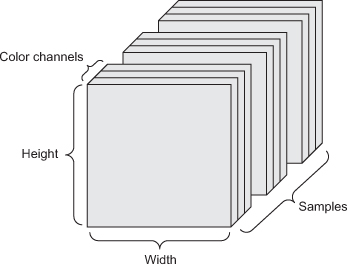
\includegraphics[width=0.6\textwidth]{Pics/image.jpg}
        \end{figure}

	\small{A batch of 128 colour images can be stored in a 4D tensor with shape \texttt{(128,256,256,3)}}

\end{frame}

\begin{frame}
        \frametitle{Anatomy of a neural network}

        \begin{figure}
                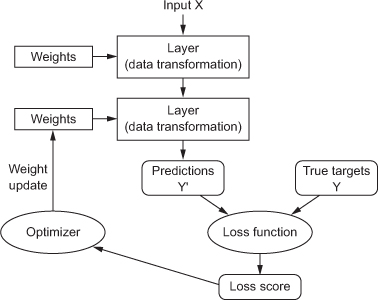
\includegraphics[width=0.5\textwidth]{Pics/nn_scheme.jpg}
        \end{figure}

\end{frame}


\begin{frame}
	\frametitle{Build your first neural network}

	\begin{enumerate}
		\item collect and preprocessing a dataset: most of the actual work
		\pause
		\item build your model: few lines of code
		\pause
		\item train: one line of code
		\pause
		\item evaluate: one line of code
		\pause
		\item predict: one line of code
	\end{enumerate}

	\bigskip
	\tiny{source: Get started with TensorFlow's High-Level APIs (Google I/O '18)}

\end{frame}

\begin{frame}
	\frametitle{Step 1: collect a dataset}

	Import the data and spend a lot of time asking questions on: rank, shape, number of objects, printing, format, data type, ...: very basic questions!


	 \begin{figure}
                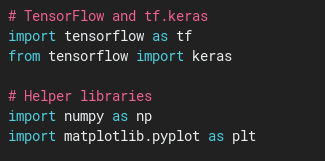
\includegraphics[width=0.6\textwidth]{Pics/tf_1.png}
        \end{figure}
	
\end{frame}

\begin{frame}
        \frametitle{Step 1: collect a dataset}

         \begin{figure}
                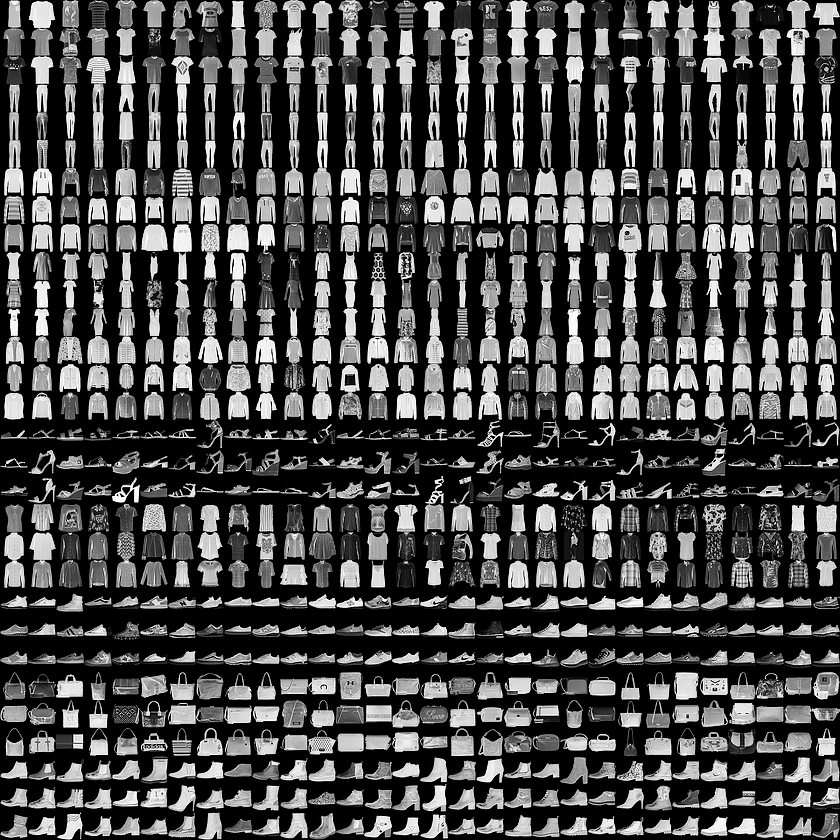
\includegraphics[width=0.4\textwidth]{Pics/fashion-mnist.png}
        \end{figure}

	\small{70,000 28x28 grayscale images in 10 categories of clothing articles}

\end{frame}

\begin{frame}
        \frametitle{Step 1: collect a dataset}

         \begin{figure}
                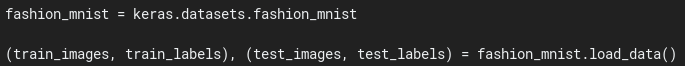
\includegraphics[width=0.9\textwidth]{Pics/tf_2.png}
        \end{figure}

	 \begin{figure}
                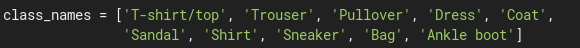
\includegraphics[width=0.9\textwidth]{Pics/tf_3.png}
        \end{figure}

\end{frame}

\begin{frame}
        \frametitle{Step 2: build a model}

	\begin{figure}
                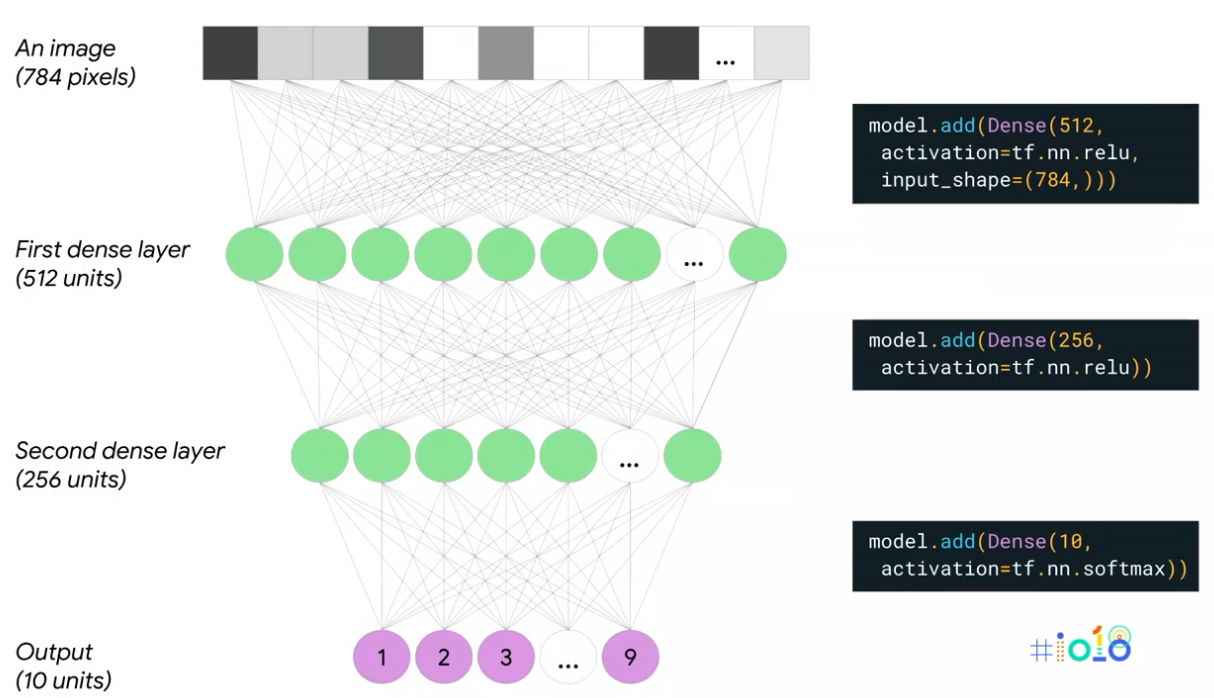
\includegraphics[width=0.9\textwidth]{Pics/nn_google.png}
        \end{figure}

\end{frame}

\begin{frame}
        \frametitle{Step 2: build a model}

	\begin{itemize}

	\item start simple! do not overlearn the training set.

	\item define loss function

	\item define optimization (important but defaults are good)

	\end{itemize}

	\begin{figure}
                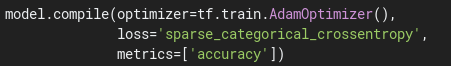
\includegraphics[width=0.9\textwidth]{Pics/compile.png}
        \end{figure}

	\small
	When you choose a network topology, you constrain your space of possibilities (hypothesis space) 
	to a specific series of tensor operations, mapping input data to output data.

\end{frame}

\begin{frame}
        \frametitle{Step 3: train the model}

	 \begin{figure}
                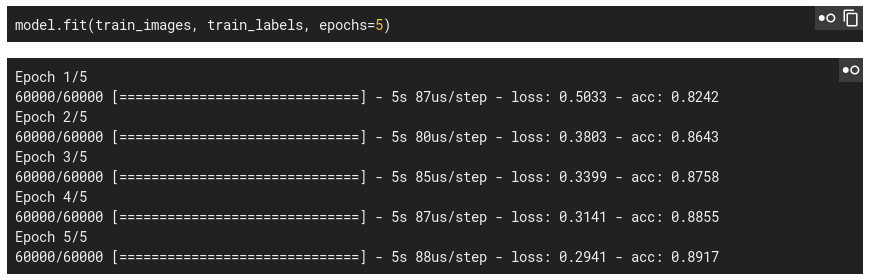
\includegraphics[width=0.9\textwidth]{Pics/train.png}
        \end{figure}

	Only "epochs" (and "batch size") matter here.

\end{frame}

\begin{frame}
	\frametitle{Step 4: evaluate}

	\begin{figure}
                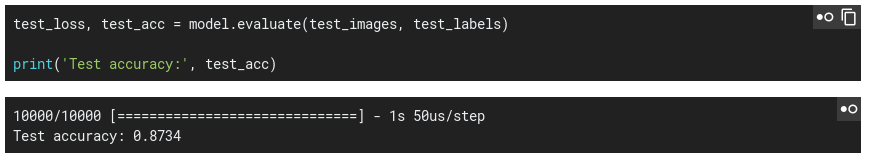
\includegraphics[width=0.9\textwidth]{Pics/evaluate.png}
        \end{figure}

\end{frame}

\begin{frame}
	\frametitle{Step 5: predict}

	\begin{figure}
                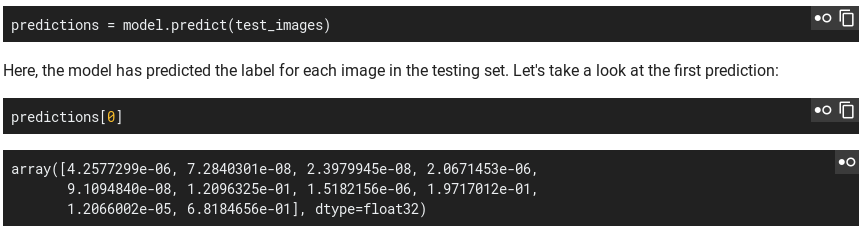
\includegraphics[width=0.9\textwidth]{Pics/predict.png}
        \end{figure}

	\url{https://www.tensorflow.org/tutorials/keras/basic_classification}

\end{frame}

\begin{frame}
        \frametitle{Keras}

         \begin{figure}
                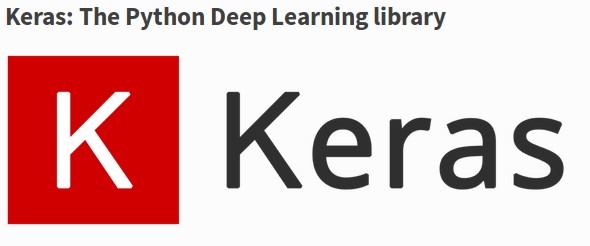
\includegraphics[width=0.6\textwidth]{Pics/keras.png}
        \end{figure}

	"Keras is a high-level neural networks API, written in Python and capable of running on 
	top of TensorFlow, CNTK, or Theano."

\end{frame}

\begin{frame}
        \frametitle{Keras}

         \begin{figure}
                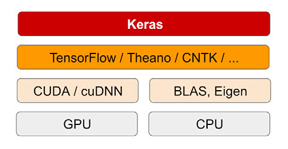
\includegraphics[width=0.5\textwidth]{Pics/keras2.jpg}
        \end{figure}

\end{frame}

\begin{frame}
        \frametitle{Population genetics}

        \begin{figure}
                        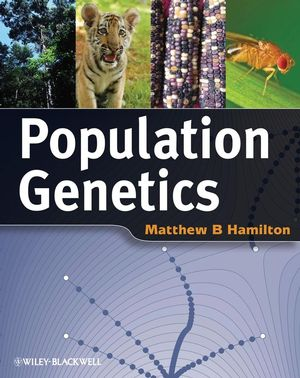
\includegraphics[height=0.6\textheight]{Pics/popgen.jpg}
        \end{figure}

\end{frame}

\begin{frame}
        \frametitle{Population genetics}

        \begin{figure}
                        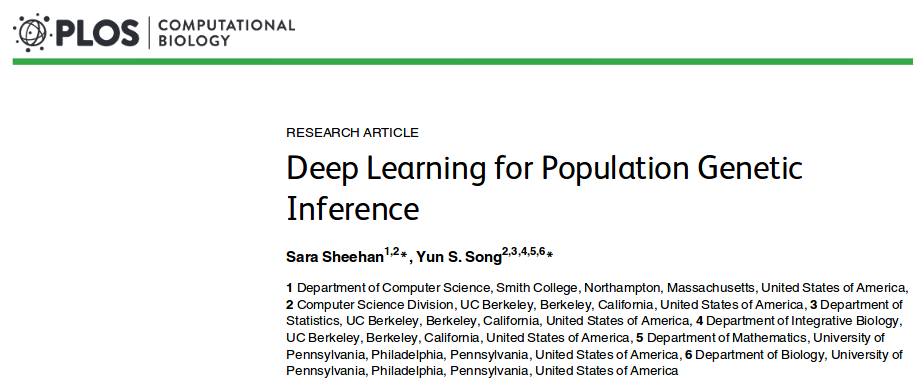
\includegraphics[width=1\textwidth]{Pics/sara.png}
        \end{figure}

\end{frame}

\begin{frame}
        \frametitle{Population genetics}

        \begin{figure}
                        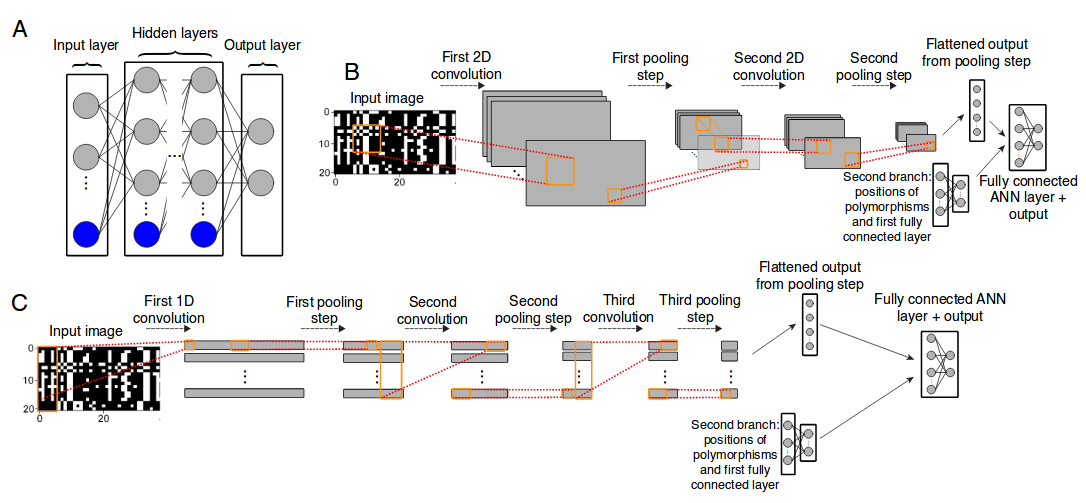
\includegraphics[width=1\textwidth]{Pics/flagel.png}
        \end{figure}

\end{frame}

\begin{frame}
        \frametitle{IUCN Red List of Threatened Species}

        \begin{columns}
                \column{0.5\textwidth}
                LC: least concern
                \begin{figure}
                        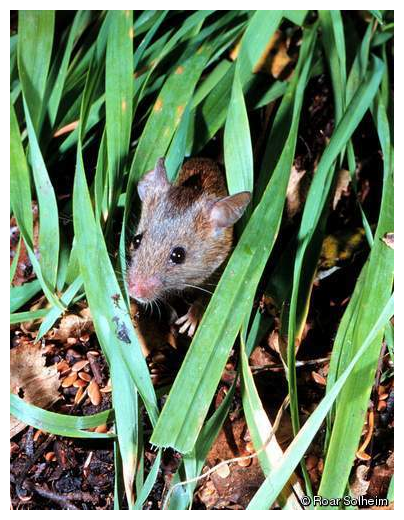
\includegraphics[height=0.2\textheight]{Pics/LC}
                \end{figure}
                VU: vulnerable
                \begin{figure}
                        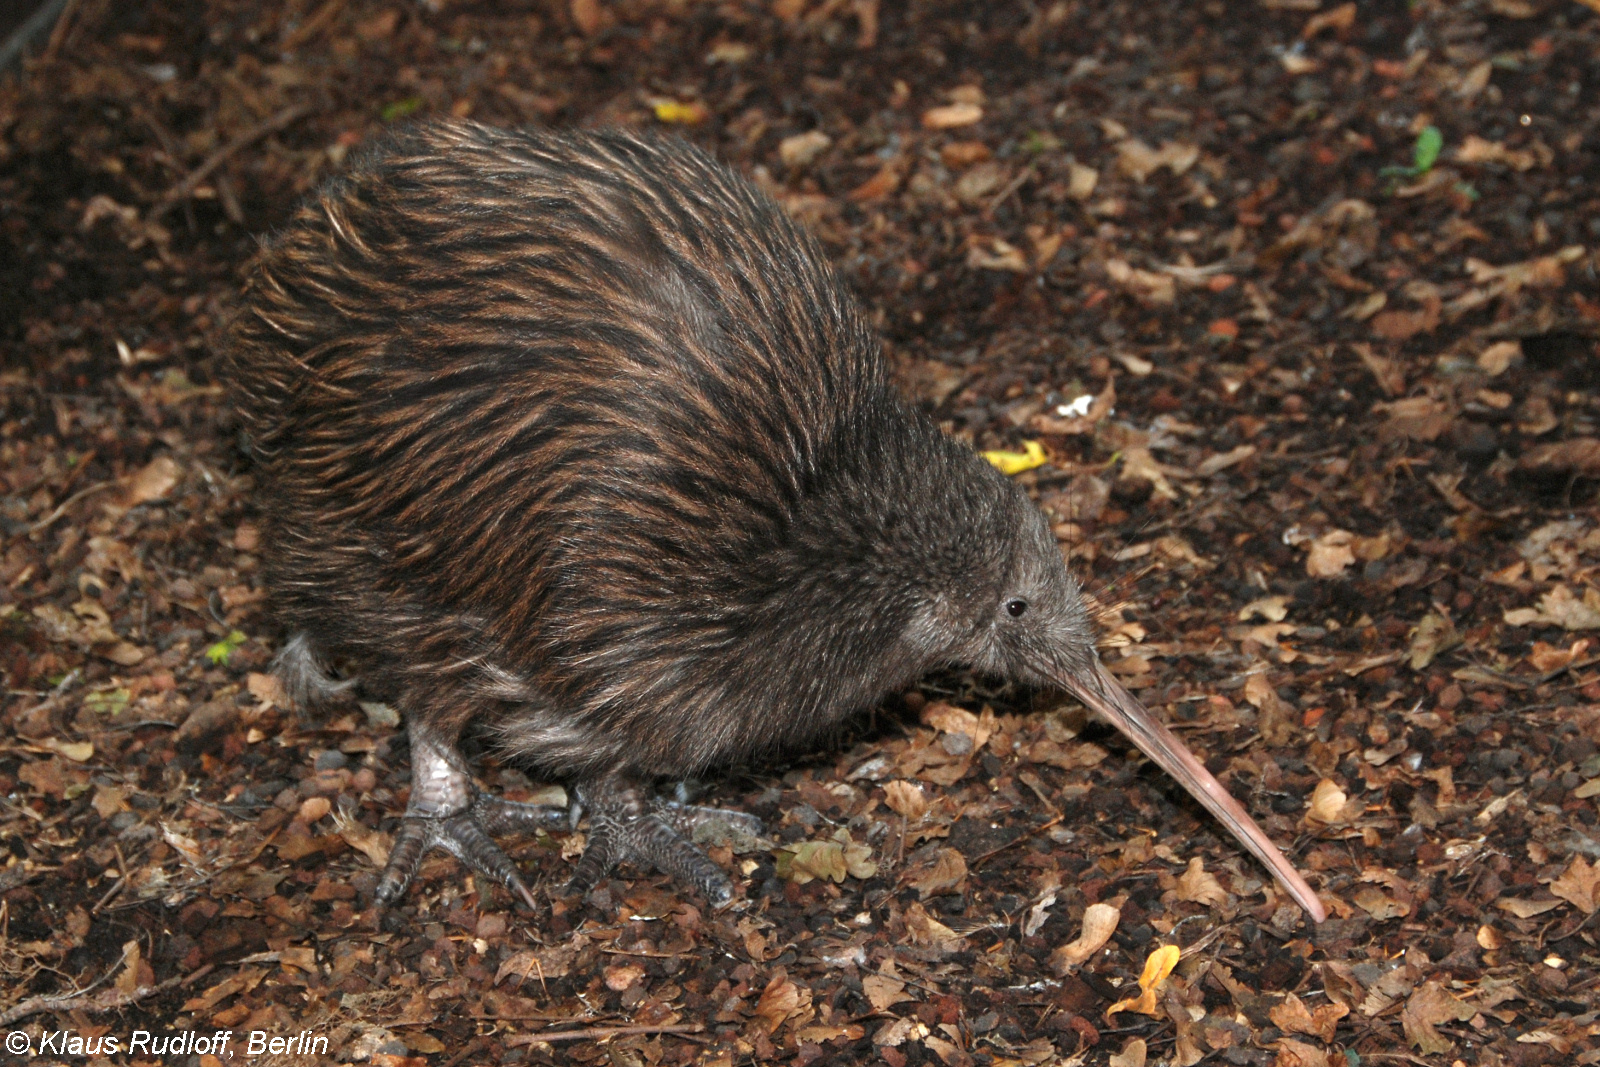
\includegraphics[height=0.2\textheight]{Pics/VU}
                \end{figure}
                \column{0.5\textwidth}
                EN: endangered
                \begin{figure}
                        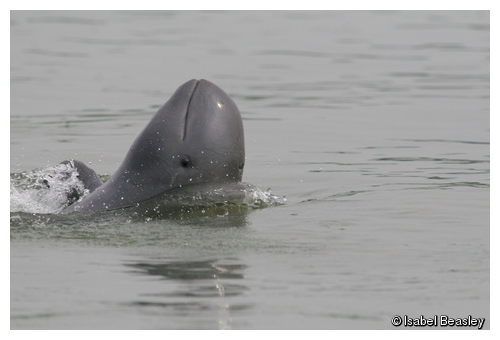
\includegraphics[height=0.2\textheight]{Pics/EN}
                \end{figure}
                CR: critically endangered
                \begin{figure}
                        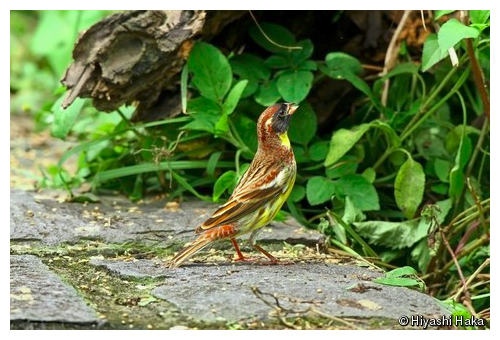
\includegraphics[height=0.2\textheight]{Pics/CR}
                \end{figure}
        \end{columns}

\end{frame}

